% Chapter 5

\chapter{Literature Study on Map Design and Data
  Visualization} % Main chapter title

\label{Chapter5} % For referencing the chapter elsewhere, use \ref{Chapter1} 

\lhead{Chapter 5. \emph{Map Design}} % This is for the header on each page - perhaps a shortened title

%----------------------------------------------------------------------------------------
\section{Overview}
This section includes case and literature studies of map design and
space time information visualization and analysis.

\section{Works on Map Design}\label{mapDesign}

\subsubsection{2D vs. 3D} \label{2d3d} 

As is mentioned in ~\cite{Brownrigg2005}, the choice of 2D
representation vs. 3d representation is one of the debating decisions
in the world of cartographic data
visualization~\cite{Brownrigg2005}. 2D maps are 1) easier to navigate
through and 2) easier to perform selection and manipulation. Another
important advantage of 2D map is that it has better theory
support~\cite{Resch2014} while the principles and variables of 3D or
4D maps (space-time map) are not thoroughly
investigated~\cite{Resch2014}. This situation makes the design of 3D
maps more difficult. However 2D maps ``drastically simplify reality
and thus do not give credit to the highly complex capabilities of
human spatial cognition''~\cite{Resch2014}. Regarding this, 3D map is
rich in geometry representation and can provide realistic scenes. This
feature can both be an advantage or disadvantage based on the actual
map usage. According to Tufte's data-ink ratio theory, the extra
non-crucial richness of information should be eliminated to make the
most important bits of information stand out~\cite{Tufte83}. Sometimes
it could better to retreat from 3D representation to 2D representation
if the third dimension add no new information to the data display and
creates too much distraction.

For the current dynamic map display, both 2D and 3D representations
are provided for the users to select. With 2D map representation,
users can select building footprints and create data plots. With 3D
map display, users are able to visualize the actual building
configuration of the community. Additional building features could be
added to make the display more realistic.

\subsection{Bivariate Map Design} \label{bivariate} 

Our major intention in choosing the 3D energy dynamic map display is
to use it to provide a more realistic urban environment context.
Although the approach of representing different energy demand and
supply sources by height, which is the approach adopted by Dobbelsteen
et al.\ ~\cite{Dobbelsteen2013}, is easier for aggregating many
different sources together, this approach is not suitable for our map
design because it creates too much shape distortion and will impair
our goal of providing a realistic urban environment vision.  In order
to represent space heating demand and cooling demand on the same map,
a common map design problem is encountered in the current project:
bivariate map design problem. Elmer presented eight possible types of
representation for bivariate maps (\fref{fig:bivariateExp}): ``shaded
cartographer, rectangle map, bar chart, value by alpha, choropleth
with graduated symbol, bivariate choropleth, spoke glyph and shaded
texture''~\cite{Elmer2012}. In order to incorporate the bivariate map
symbols to the current 3D model without introducing too much shape
distortion, the representation with dimensional changes are not
chosen. The only choices are the ones that only involves color or
texture, i.e. ``bivariate choropleth, value by alpha and shaded
texture''. Among these three choices, bivariate choropleth
representation has the highest accuracy rate~\cite{Elmer2012}, hence
we choose bivariate choropleth as the representation of the current
map interface design.

\begin{figure}[h!]
  \centering
  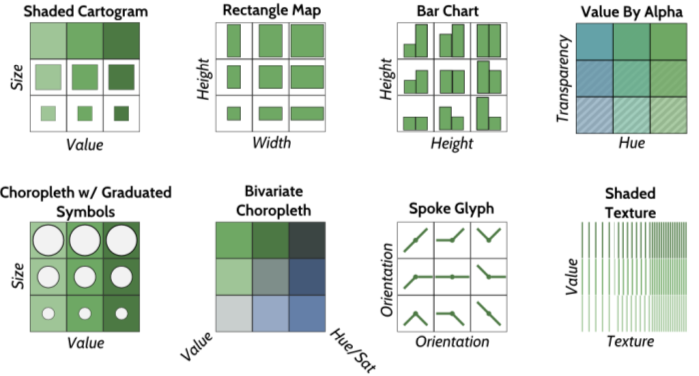
\includegraphics[width=0.7\linewidth]{bivariateExp.png}
  \caption[Bivariate Map Symbol Tested]{The eight bivariate map
    display approaches tested in Elmer's~\cite{Elmer2012} study}
  \label{fig:bivariateExp}
\end{figure}

\section{Works on Dynamic (Space-time) Map Design}\label{mapDesign}

Dorling and Openshaw pointed out that dynamic map provide new
potential and possibilities for data analysis but also pose a great
challenge as a result of the less developed theory in space-time
pattern detection and measurement~\cite{Dorling1992}. In order to
better conduct a space-time visualization of the space-time energy
demand information in the dynamic energy map, we conducted some
literature studies on space-time map visualization.

\subsection{Symbol Chosen}\label{symbolChosen}
Dong et al.\ assessed the effectiveness of symbol design and frame
rate on the effectiveness of dynamic map display with two performance
measurements: deviation and response time. They discovered the change
of symbol size is more effective than color under the same frame
rate. They also identified the optimal class numbers is 15 for
graduated size symbol and is 10 for graduated color symbol on a
1024x768 display. The optimal frame rate identified in the study is 3
for color symbol maps and 6 for size symbol maps. They also suggest to
reduce class number and frame rate if the display size is smaller than
1024x768~\cite{doi:10.1559/1523040639298}. 

For the current dynamic energy map, the display size is $600 x 300$,
less than the $1024 \times 768$, thus we chose 7 classes for data
classification. The interactive animation (the interface with sliders)
has map display of size $600 \times 300$, if displayed as animation,
the frame rate should probably be about 2 per second according to the
findings in ~\cite{doi:10.1559/1523040639298}. The non-interactive
animated map display has size of $1213 \times 950$, a little larger
than that of the suggested display, we thus chose the frame rate to be
4 per second.

\subsection{Time Representation}\label{timeRepresent}
Brownrigg mentioned several methods of representing time on a map: 1)
a graph or chart that represents a function over time or a time line
for displaying chronological events 2) animation of snapshots
(animated map) 3) small-multiples of snapshots of changing states
~\cite{Brownrigg2005}.

Based on the classification above, the current interface design
applied method 1) and 2) in time representation. The dynamic plot of
temporal time series is using method 1) to anchor the quantitative
information. The interactive animation approach is using method 2) for
choropleth map display, as is apposed to method 3)(small-multiple
method). The choice is based on the following points mentioned by
Brownrigg: 1) the number of snapshots in one display is limited and
the finer the detail per snapshot, the less snapshots one can contain
in one display. Since the 3D representation is chosen as one of the
major map display methods (2D map is also available), the level of
details per image is high, which will result in a very small number of
multiples per display~\cite{Brownrigg2005} 2) the subtle changes are
easier to be noticed in the form of animation than with
small-multiples (?). Both drawbacks of small-multiple method will
impair the ability of conveying the rapid temporal changes of energy
behavior, hence is not suitable for the current project.

They also suggest the necessity of providing ``temporal context'':
``To comprehend how drastically or subtly something is changing, how
fast or slow, in what direction, in relative to its environment, etc.,
demands some knowledge of the history of the change, an awareness of
the objects' properties before and after the
change.''~\cite{Brownrigg2005}. To provide the temporal context, the
map display is accompanied with energy data plots of single buildings,
building groups and the total community, so that the viewers will have
a general understanding of whether the changing of energy demand
behavior is drastic or subtle and whether a drastic change is coming
and whether the current demand is high, low or moderate comparing to
the overall distribution over time and space (need to implement).

\subsection{Animated Maps}\label{anime}
Animated maps are proven to be more powerful in conveying the
spatial-temporal pattern than static maps~\cite{McEachern1998}.

In order to represent dynamic geographic processes, map animation is a
natural choice. It was introduced to the world of cartography in
1930s~\cite{Harrower2008}. The major application of animated maps
include: 1) demonstrating the dynamic process of geographic events
(weather maps in weather forecasting is such an example) 2) assisting
pattern recognition and knowledge development for scientific
researches. The study by Dorling and Openshaw is an example of 
application 2), where they discovered new leukaemia hotspots through
animated maps~\cite{Dorling1992}.

Animated maps are not superior to static maps, it is just they are
good at different aspects of information convey. The animated map is
advantageous in demonstrating the changes between frames rather than
the absolute value represented in each frame~\cite{Dorling1992}. It is
proved to be more powerful in convey the spatial-temporal pattern than
static map~\cite{McEachern1998}.

Harrower and Fabrikant mentioned that the chanllenge of using animated
maps is the overflow of information and the vulnerability to
distraction~\cite{Harrower2008}. One example mentioned by Harrower and
Fabrikant is the comparison of color on the map and that on the legend
becomes difficult for animated maps as a result of the changing of
images. They proposed the audio legend approach of strengthening
information convey with minimized
distraction~\cite{Harrower2008}. This might become one of the next
extensions of the current Dynamic Energy Map interface design.

They also suggested that the difference in time should have different
visual representations in data display~\cite{Harrower2008}. Peuquet
claimed that ``The development of temporal analytical capabilities in
GIS such as temporal queries requires basic topological structures in
both time and space''~\cite{Peuquet1994}. Thus the different spatial
representation seems to be a natural choice for adapting to different
temporal resolution and scale.

They classify time into two types: linear and cyclic. Upon this
consideration, the design of the current interface include both an
overall time navigation utility and time navigation utilities that
facilitate jumps with time steps corresponding to the natural period
of energy data, such as month, day and hour. This design choice
is anticipated to facilitate the representation of both linear changes
and periodical changes of energy usage in the community.

The level of user control of playback behavior of animated maps is
also debatable. Some claim providing the full freedom of adjusting
this feature can enhance pattern understanding~\cite{Nelson1998}. But
others argue that this control will reduce time animation to still
images and impair its ability in conveying temporal changes
~\cite{Lowe2004}. In the current dynamic map project, both the
interactive version and the non-interactive version is provided: the
non-interactive version (a map animation) is accessible through
\href{http://www.armechxyj.com/energy-mapping.html#redblueAnime3d}{here}. The
interactive version is provided as a stand-alone Python program.

\begin{comment}
\subsection{Spatial Temporal Data Analysis}\label{stDataAnalysis}
In order to better utilize the power of Dynamic Maps, one has to
understand the special features of spactial-temporal data and the
methods of how to use spactial-temporal data. This leads to the
literature study of the following section of spatial temporal data
analysis.

One temptation of analyzing spatial-temporal data is to aggregate them
into ``time periods'' and ``zonal entities'' and then use the static
analysis method to analyze the aggregated data~\cite{Dorling1992}. The
problem of this approach is 1) it increases the sensitivity
(i.e. minor changes in input causes dramatic changes in output) and 2)
it removes the ``dynamic'' feature of a dynamic.
map~\cite{Dorling1992}.

One layer of the goal of a space-time map is to make ``complex dynamic
process'' visible, in the hope of letting observers comprehend the
dynamics of data presented and to gain a general insight. Baring this
goal in mind, Dorling and Openshaw suggested a noise removal or data
smoothing in both the time and space dimension before the actual map
creation~\cite{Dorling1992}.
\end{comment}

\section{Data Classification}\label{dataClassification}
In order to write the data classification routine for the
demonstration of dynamic energy map in the current study, the authors
conducted a brief survey of the commonly used GIS software for
commonly applied data classification method. The software surveyed in
the study include: ArcGIS~\cite{GIS_Jenks2014}, GRASS
GIS~\cite{GRASSGIS2008}, gvGIS~\cite{gvGIS2011}, and QGIS. The data
classification method adopted by the surveyed software in creating a
thematic map include: 1) equal interval, 2) quantile 3) Jenks 4)
Standard Deviation 5) pretty breaks 6) manual interval (use context
specific break point values). The common data classification method
shared by all surveyed instances are ``Equal Interval'', ``Quantile''
and ``User Defined''. Therefore we chose to implement the ``Equal
Interval'' and ``Quantile'' method in the current project.

\begin{table}[h!]
  \centering
  \begin{tabular}{r|c c c c c c}
    \hline
           & Equal Interval & Quantile & Jenks & Pretty Breaks & StDev & User Defined\\
    \hline
    ArcGIS &      o        &    o     &  o    & x &  o  &   o  \\
 GRASS GIS &      o        &    o     &  x    & x &  o  &   o  \\
     GVSIG &      o        &    o     &  o    & x &  x  &   o  \\
      QGIS &      o        &    o     &  o    & o &  o  &   o  \\
    \hline
  \end{tabular}
  \caption{Data Classification Method (o: yes, x: no)}
  \label{tab:classify}
\end{table}

\begin{comment}

``Data Visualization with Spacetime Maps'', Richard L. Brownrigg, 2005
(read further later on)

\grey{To be continued later:
\begin{enumerate}[label*=\arabic*.]
\item ``Geographic Visualization: Designing Manipulable Maps for
    Exploring Temporally Varying Georeferenced Statistics'', MacEachren et al.\
\item ``Strategies for the Visualization of Geographic Time-Series
    Data'', Mark Monmonier, 2011
\item ``Evaluation of Methods for Classifying Epidemiological Data
    on Choropleth Maps in Series'', Brewer and Pickle, 2002
\end{enumerate}}
\end{comment}